%!TEX root = ../main.tex

\chapter{Design and Implementation}
This chapter is describes the process of producing and optimising the main component of the artefact --- the URL classifier. The first section of the chapter presents the findings of Google Safe Browsing's evaluation, the result of which constitutes the minimum acceptable classification accuracy.

The following two sections briefly describe the list-based module and explores machine-learning module of the artefact. Next, an initial performance analysis is carried out which sets the scene for further optimisation. Finally, the aforementioned components are brought together and assessed as a whole.

\section{Threshold definition}
Before attempting to improve the level of protection offered by the most popular browsers, Google Safe Browsing's effectiveness needs to be assessed. In doing so the behaviour of the user will be simulated using an browser automation framework for accessing the confirmend phishing websites. The outcome of this serves as an accuracy threshold for the proposed artefact.

The first step of the process is data aquisition. A list of URLs pointing to online phishing webpages, confirmed to be malicious by the PhishTank community is fetched from their archive. The first test is run on the data available on the 1st on April. Testing a total number of 9345 phishing URLs, Google Safe-Broswing managed to achieve a total accuracy of 50.76\%.
The next test is run with the data published on the 7th of April. This time Google Safe-Browsing performed slightly worse reporting an accuracy of 48.32\% on the 8164 phishing URLs. Running the same test on the data aquired on the 1st of April shows a significant drop in accuracy, reporting an accuracy of 40.28\% on a number of 9359 URLs.
One important mention is that because Google Chrome is rather resource demanding software, the results are altered by the fact that the testing phase of a dataset takes around eight hours. In this time Chrome has opportunities to update it's database of malicious websites.

Shifting the testing method to Google Safe Browsing API, the protection rate is slightly lower (Table \ref{tab:GSBAPI_RESULTS}). Finally, the threshold is set to be the average of all test results of 45.74\%.


\begin{singlespace}
	\small
	\begin{table}
		\begin{center}
			\label{tab:GSBAPI_RESULTS}
			\begin{tabular}{ | m{8em} | m{13em} | }
				\hline
				\textbf{Date}        & \textbf{True-positive rate} \\
				\hline
				\textbf{05 May 2020} & 44.34\%                     \\
				\hline
				\textbf{05 May 2020} & 44.33\%                     \\
				\hline
				\textbf{05 May 2020} & 44.94\%                     \\
				\hline
				\textbf{05 May 2020} & 45.34\%                     \\
				\hline
				\textbf{05 May 2020} & 45.33\%                     \\
				\hline
				\textbf{05 May 2020} & 43.60\%                     \\
				\hline
			\end{tabular}
			\caption{Google Safe Browsing API test results}
		\end{center}
	\end{table}
\end{singlespace}


\section{List based module}
It is safe to assume that most of web browsing activity takes place across a limited set of domains. This is reflected in the existence of domain rankings of most popular domains. Because these are known to be benign, there is no reasong for wasting resources on the classification process. Because of this, a list based module is included in the phishing detection system.
The white-list included is comprised of the domains ranking published by \cite{MAJESTIC_MILLION}.

\section{Machine learning module}
As the current literature shows, there is a breadth of approaches in detection and prevention of phishing attacks. However, an emergent pattern in effective anti-phishing detection systems is the use of machine learning. A well trained and optimised module of this kind increases the performance and robustness of the proposed artefact. Besides this, it offers the capability of dealing with newly registered phishing domains and URLs without further training.

\subsection{Features exploration}
The features selected for extraction are the cornerstone of well developed model. Because these serve to emphasise on areas where the two classes of URLs differ, most of the effort should go in carefuly building the feature set. The aim of this subsection is to find correlations that best separate benign URLs from phishing ones. As this artefact competes with the most popular phishing detection system, the dataset is chosen to be comprehensive in virtually all aspects.

The feature selection process starts with URL length. The literature is quite clear on the discrepancy in average URL length between legitimate and phishing URLs. One example is illustrated by \cite{STACKED_ML_URL_HTML} (Figure \ref{fig:URL_LENGTH_DISTRIBUTION}), showing the length distribution over a set of 50,000 URLs. Doing a URL length analisys (Table \ref{tab:URL_SIZE_ANALISYS}) on the dataset used in training the artefact, there is an obvious correlation between maliciousness and URL length.

\begin{figure}[t]
	\centering
	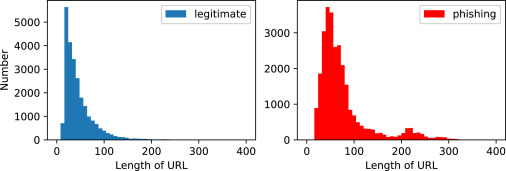
\includegraphics[width=0.9\textwidth]{url_length_50k.jpg}
	\caption{URL length distribution over a dataset of 50,000 records}
	\label{fig:URL_LENGTH_DISTRIBUTION}
\end{figure}

\begin{singlespace}
	\small
	\begin{center}
		\label{tab:URL_SIZE_ANALISYS}
		\begin{tabularx}{\textwidth}{ | X | X | X | }
			\hline
			                         & \textbf{Benign} & \textbf{Phishing} \\
			\hline
			\textbf{Average}         & 57.81           & 77.54             \\
			\hline
			\textbf{Median}          & 52              & 52                \\
			\hline
			\textbf{90th percentile} & 90              & 147               \\
			\hline
			\textbf{95th percentile} & 107             & 220               \\
			\hline
			\textbf{99th percentile} & 141             & 321               \\
			\hline
		\end{tabularx}
		\captionsetup{type=table}\caption{Statistical analysis of URL length over the training dataset}
	\end{center}
\end{singlespace}


The second feature selected is the protocol used. There is a case to be made against using protocol as a feature due to its rise is usage shown by the \cite{APWG_Q42019}. However, although TLS adoption is growing, serving a website through HTTPS requires technical knowledge and a certain amount of effort. Besides this, the low average lifespan of a phishing webpage could help the average attacker decide against using it. Based on these factors it is safe to assume that the number of phishing websites using TLS will not exceed 85\%. As of now, Doing protocol analisys on the dataset shows that the lack of TLS usage and maliciousness are highly correlated (Figure \ref{fig:FEATURE_CORRELATION}).

The third feature selected is the number of numerical characters in both the domain and subdomain. The choice comes from the fact that it is highly uncommon for benign domains and especially subdomains to contain any digits.

The fourth feature is the number of '@' and '~' characters. The reasoning behind this is that, like numerical characters, it is uncommon for an URL to contain these characters. The tilde is an outdated practice of accessing a user's folder on a linux system by appending their name after the '~' character.
The '@' is especially dangerous as it produces unexpected behaviour in the browser. It could either redirect to an email address using the default mail client or get the browser to ignore every character on it's rigth side.

The analysis of the dataset (Figure \ref{fig:FEATURE_CORRELATION}) shows that although they do not occur as often, these characters are still indicative of malicious activity and can improve decision-making.

The fifth feature is the presence of an additional network location in the URL. Given the popularity of hosting or storage services today and the existence of many open redirect vulnerabilities, some phishing URLs hide their real domain behind the trusted domain of another company. This feature flags up the presence of such practice by checking if the number of dots in the path of the URL exceeds one.

The sixth feature chosen is the number of hyphens. If there is no domain present in the path portion of the URL, the hyphen count is determined based on the network location only, otherwise for the whole URL. This is done to cover cases such as "target-brand.example.com" and "storage.service.com/website/target-brand.example.com/"

The seventh feature selected is the number of subdomains components. Most of benign URLs either use "www" as subodmain, or another arbitrary string of characters. But the thing they have in common is that they mostly use only one subdomain component. Phishing URLs however, may use a multi-component subdomain to create the illusion of the target brand. Based on this reasoning, this feature will flag any URL whose subdomain components count exceeds two.

The eighth, nineth and tenth features flag the presence of sensitive vocabulary in the URL. \cite{10.1145/1314389.1314391} uncovered the correlation between a set of "sensitive" words and malicious intent in the study of phishing URL obfuscation techniques. The study has been done in 2007, so in order to maximize the efficiency of the word set, it needs to be extracted from an updated set.
The word frequency count is performed on a coroboration of multiple Phishtank lists of valid phishes. These are split in the format of <subdomain>.<domain>/<path>?<query> and further probabilistically split concatenated words using natural language processing (NLP) based on English Wikipedia unigram frequencies.

Visual exploration of the sensitive vocabulary of the query segment shows that it overlaps with the one used in benign URLs, thus being prone to causing numerous false positives. Because of this, the final lists of sensitive words used are for the subdomain, domain and path section.

To further enhance the potential of this feature, the path and query sections of the URLs are searched for popular domains. Because it is a common practice in phishing URLs to use the target domain or brand in the path under the form of "www.example.com/brand/signin.html", if there is no sensitive word found in path, the first 2500 domains are searched throughout the path and query portions.

The last two features are based on the similarity index between URL's domain and subdomain, and the top N benign domains. This feature directly targets the practice of brand obfuscation through variations creating the surface illusion of accessing a trusted domain.
Phishing URLs use an array of techniques to create this illusion. A comprehensive list of these mutations is presented in Table \ref{tab:VARIATIONS_EXAMPLE}. All these permutations are done with the aim of tricking the viewer if they're not exercising a closer inspection.

\begin{singlespace}
	\begin{center}
		\label{tab:VARIATIONS_EXAMPLE}
		\begin{tabular}{ | m{13em} | m{13em} | }
			\hline
			\textbf{Method}        & \textbf{Example result} \\
			\hline
			\textbf{Original}      & example.com             \\
			\hline
			\textbf{Addition}      & examplea.com            \\
			\hline
			\textbf{Bitsquatting}  & azample.com             \\
			\hline
			\textbf{Homoglyph}     & ēxãmple.com             \\
			\hline
			\textbf{Hyphenation}   & exampl-e.com            \\
			\hline
			\textbf{Insertion}     & examplme.com            \\
			\hline
			\textbf{Omission}      & exaple.com              \\
			\hline
			\textbf{Repetition}    & exxample.com            \\
			\hline
			\textbf{Replacement}   & esample.com             \\
			\hline
			\textbf{Subdomain}     & ex.ample.com            \\
			\hline
			\textbf{Transposition} & exapmle.com             \\
			\hline
			\textbf{Vowel-swap}    & exomple.com             \\
			\hline
			\textbf{TLD inclusion} & examplecom.com          \\
			\hline
		\end{tabular}
		\captionsetup{type=table}\caption{Domain variation techniques}
	\end{center}
\end{singlespace}

To capture such patterns feature 10 measures the Levenshtein distance between the target URL and the top 25,000 benign domains. The Levenshtein distance quantifies the difference between two strings by calculating the number of operations (deletion, insertion and substitution) needed to be performed on one of the strings for them to become identical. In case the Levenshtein distance is lower than six and different than zero, then the URL is flagged as suspicious. 

The next feature applies the same process but on the extracted subdomain components. In this case a distance lower than three will flag up the URL as suspicious. This is because subdomains closer to popular domain names are more suspicious than different variations of a domain.

Looking at the correlations between the label (benign or malicious) and the feature set presented in this section (Figure \ref{fig:FEATURE_CORRELATION}) we can see how popular these practices are.

\begin{figure}[t]
	\centering
	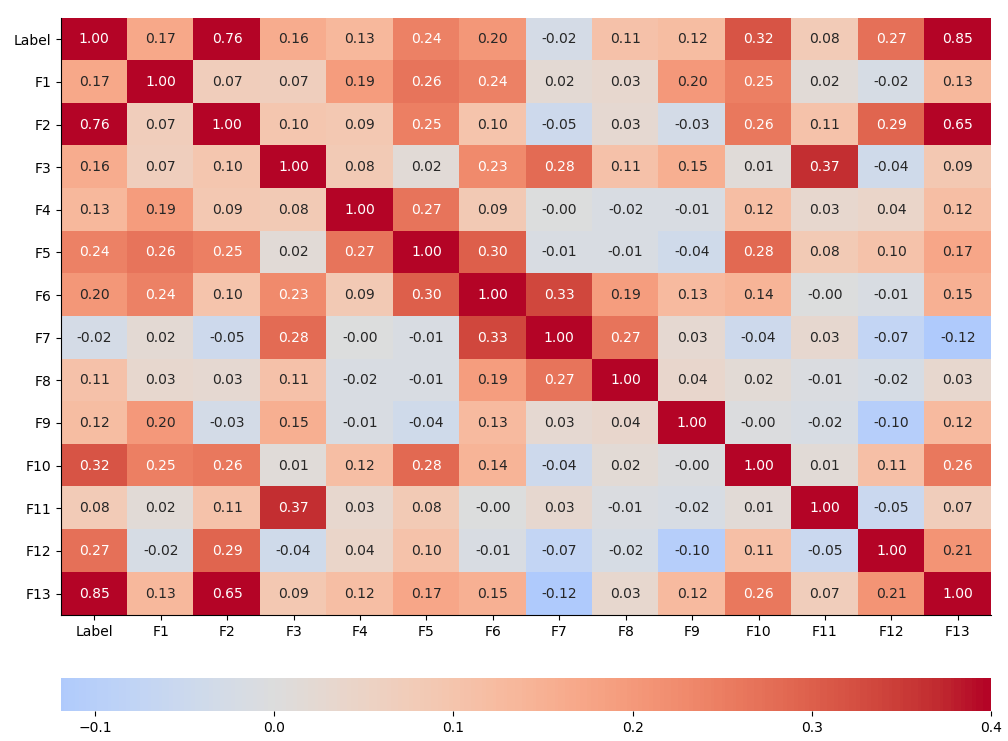
\includegraphics[width=1\textwidth]{feature_correlation.png}
	\caption{Correlation between labels and features}
	\label{fig:FEATURE_CORRELATION}
\end{figure}

\section{Initial performance assessment}
This section follows the process of model training and initial performance assessment. The results of training the first set of models shows great synergy between the features. Table \ref{tab:FIRST_TRAINED_MODELS} presents the F1 scores of the alorightms. The F1-score is the chosen as metric because it is suitable to generalize performance.

\begin{singlespace}
	\begin{center}
		\label{tab:FIRST_TRAINED_MODELS}
		\begin{tabular}{ | m{13em} | m{13em} | }
			\hline
			                                & \textbf{F1-score} \\
			\hline
			\textbf{Naive Bayes}            & 98.37\%           \\
			\hline
			\textbf{Decision Tree}          & 98.74\%           \\
			\hline
			\textbf{Random Forest}          & 98.86\%           \\
			\hline
			\textbf{Support Vector Machine} & 98.76\%           \\
			\hline
			\textbf{Multi-layer Perceptron} & 97.21\%           \\
			\hline
		\end{tabular}
		\captionsetup{type=table}\caption{F-measure results of models training}
	\end{center}
\end{singlespace}

Figure \ref{fig:ROC_CM_EXAMPLE} presents both the ROC and confusion matrix for the Random Forest model. The maximum area under curve (AOC) shows that the model can easily distinguish between the two types of URLs. The confusion matrix shows that it is uncommon for the algorithm to mislabel URLs. In the example the random forest mislabeled 109 URLs out of 10,000.

To test its performance in a realistic scenario, the models are set to deliver predictions on the remainder benign and phishing URLs of the 450,000 dataset. The results collected from the predictions over 305,737 benign URLs and 74,436 phishing urls are presented in Table \ref{tab:FIRST_TRAINED_MODELS}.


% NEEDS TO BE RERUN
\begin{singlespace}
	\begin{center}
		\label{tab:FIRST_TRAINED_MODELS}
		\begin{tabular}{ | m{13em} | m{5em} | m{5em} | m{5em} | m{5em} | }
			\hline
			                                & \textbf{Precision} & \textbf{Sensitivity} & \textbf{F1-score} & \textbf{Accuracy} \\
			\hline
			\textbf{Naive Bayes}            & 89.86\%            & 99.28\%              & 94.34\%           & 97.66\%           \\
			\hline
			\textbf{Decision Tree}          & 95.10\%            & 99.12\%              & 97.07\%           & 98.83\%           \\
			\hline
			\textbf{Random Forest}          & 94.71\%            & 88.17\%              & 96.89\%           & 98.75\%           \\
			\hline
			\textbf{Support Vector Machine} & 94.88\%            & 99.16\%              & 96.97\%           & 98.78\%           \\
			\hline
			\textbf{Multi-layer Perceptron} & 19.57\%            & 100\%                & 32.74\%           & 19.57\%           \\
			\hline
		\end{tabular}
		\captionsetup{type=table}\caption{Initial models tested on 380,173 mixed URLs}
	\end{center}
\end{singlespace}


The next dataset used to evauate model performance is composed of online and valid phishes from 1st of April. This way the models are tested on the same parameters Google safe browsing was.

\begin{singlespace}
	\begin{center}
		\label{tab:FIRST_TRAINED_MODELS}
		\begin{tabular}{ | m{13em} | m{5em} | m{5em} | m{5em} | m{5em} | }
			\hline
			                                & \textbf{Precision} & \textbf{Sensitivity} & \textbf{F1-score} & \textbf{Accuracy} \\
			\hline
			\textbf{Naive Bayes}            & 100\%              & 83.33\%              & 90.91\%           & 83.33\%           \\
			\hline
			\textbf{Decision Tree}          & 100\%              & 81.15\%              & 89.59\%           & 81.15\%           \\
			\hline
			\textbf{Random Forest}          & 100\%              & 82.11\%              & 90.17\%           & 82.11\%           \\
			\hline
			\textbf{Support Vector Machine} & 100\%              & 78.91\%              & 88.21\%           & 78.91\%           \\
			\hline
			\textbf{Multi-layer Perceptron} & 100\%              & 82.69\%              & 90.52\%           & 82.69\%           \\
			\hline
		\end{tabular}
		\captionsetup{type=table}\caption{Initial models tested with Phishtank data (1st of April)}
	\end{center}
\end{singlespace}


\section{Performance improvement}
Given the results of the models presented in the previous section, the performance improvement shown in this section is not expected to be substantial.
The first step in improving the performance is removing features with a correlation to the label close to zero. The correlation heatmap presented in Figure \ref{fig:FEATURE_CORRELATION} shows feature number seven as having the lowest correlation to the label. Removing the long subodmain feature reduces confusion in model training and offers a slight improvement in delivering more accurate predictions. Figure \ref{fig:IMPROVED_FEATURE_CORRELATION} illustrates the correlation heatmap after removal.

\begin{figure}[t]
	\centering
	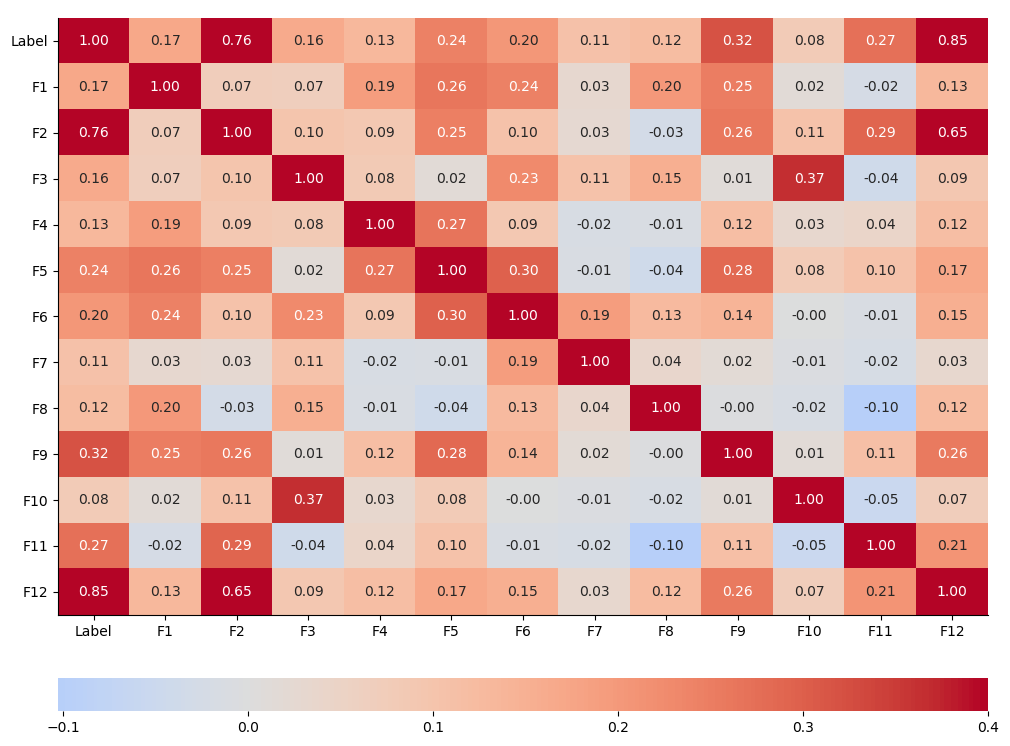
\includegraphics[width=1\textwidth]{improved_feature_correlation.png}
	\caption{Improved feature correlation heatmap}
	\label{fig:IMPROVED_FEATURE_CORRELATION}
\end{figure}

The second step is hyperparameter tuning. The process of hyperparameter tuning or optimisation consists of training the subject model with different values for it's parameters. Trying different permutations of values for these parameters influences prediction accuracy, thus finding the right combination improves overall performance.

Hyperparameter tuning is resource expensive. Because of this, the algorithms selected for optimisations are the ones that already deliver good and consistent results. These are the random forest, the support vector machine and the multi-layer perceptron classifiers.

The calibration is done using GridSearchCV. GridSearchCV does and exhaustive search over specified parameters and selects the best performing model.

Starting with the optimisation of the random forest classifier, the number of n\_estimators is increased to raise the number of decision trees. By doing so the model can delivers better predictions at the expense of both training an prediction time. Because of this the number of n\_estimators is set to either 150, 295 or 350. Next the max\_depth of each decision tree is set to be either 15,18 or 21. The last optimisation is done on the max\_features parameter. This sets the number of maximum features provided to each tree and will be tested with the values of auto and sqrt.

The calibration of the SVM classifier is done by searching for the best performing C parameter. The C parameter influences the missclassification threshold of the model. With a greater C value, the classifier will chose a smaller-margin hyperplane, rendering the model less prone to delivering wrong predictions. However, a bigger C value will increase the chance of overfitting. Because of that, the values of the C fed into the GridSearchCV are 10,100 and 1000.

Given the opaque nature of the training process of neural networks, the calibration of the multi-layer perceptron resembles hit-or-miss experimentation. Because of this, different models have been trained using most of the optimisation parameters that the MLP classifier takes as input (REF TO ANNEX).

\begin{singlespace}
	\begin{center}
		\label{tab:OPTIMISED_MODELS}
		\begin{tabular}{ | m{13em} | m{5em} | m{10em} | m{2.3em} |}
			\hline
			                                & \textbf{F1-score} & \textbf{F1-score (optimised)} & \textbf{Delta} \\
			\hline
			\textbf{Random Forest}          & 98.86             & 98.92                         & 0.08           \\
			\hline
			\textbf{Support Vector Machine} & 98.76             & 98.87                         & 0.11           \\
			\hline
			\textbf{Multi-layer Perceptron} & 97.21             & 98.76                         & 1.25           \\
			\hline
		\end{tabular}
		\captionsetup{type=table}\caption{Comparison of optimised models}
	\end{center}
\end{singlespace}


\begin{figure}[!b]
	\centering
	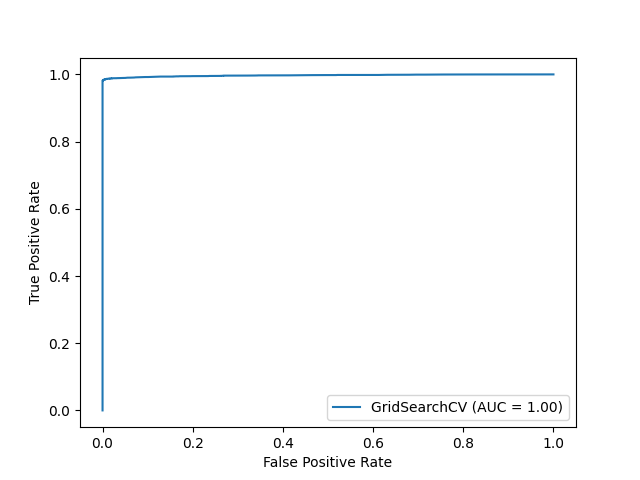
\includegraphics[width=0.49\textwidth]{random_forest_calibrated_roc.png}
	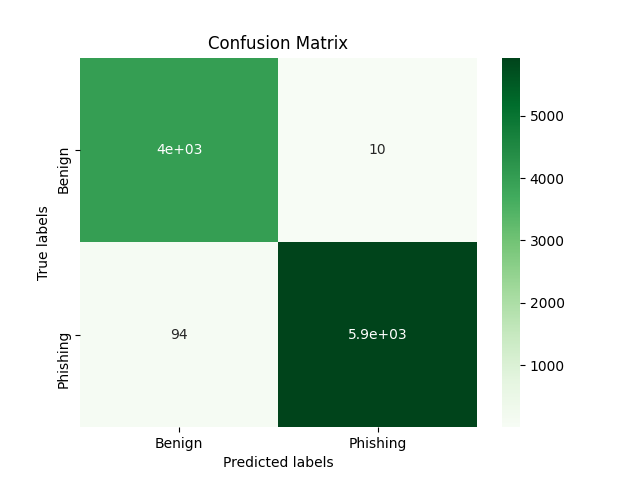
\includegraphics[width=0.49\textwidth]{random_forest_calibrated_cm.png}
	\caption{ROC and confusion matrix of the random forest model}
	\label{fig:OPTIMISED_RF}
\end{figure}

As expected, the results of the optimisation did not deliver a substantial improvement. Table \ref{tab:OPTIMISED_MODELS} shows that the best model to include in our final classifier is random forest. But before venturing to do so, additional testing needs to be perform to ensure the model is not overfitted. For this, the remainder of the initial dataset is used. Table (REF) shows that not only the model is not overfit, but the accuracy is higher by 0.35\% than the one reported during training.



\begin{singlespace}
	\begin{center}
		\label{tab:OPTIMISED_MODELS}
		\begin{tabular}{ | m{8em} | m{5em} |}
			\hline
			\textbf{Precision}   & 97.40\% \\
			\hline
			\textbf{Sensitivity} & 99.06\% \\
			\hline
			\textbf{F-measure}   & 98.22\% \\
			\hline
			\textbf{Accuracy}    & 99.29\% \\
			\hline
		\end{tabular}
		\captionsetup{type=table}\caption{ Optimised random forest results on the 380,000 records dataset}
	\end{center}
\end{singlespace}



An important factor in model selection and calibration is the amount of false positives produces. It is safe to assume that the higher the delivery of false positives, the less the alerts are taken into consideration by the user. Because of this the final model needs to prioritise precision over recall and false negatives over false positives.

The confusion matrix (Figure \ref{fig:OPTIMISED_RF}) proves that the final random forest model fulfils this aim by having a 0.10\% rate of false positives.


%=========================================================================================================
% Skipped compiling instructions
\iffalse
	You should always start with an overview (Heading 2 style) to tell what this chapter is about and finish with a summary (Heading 2 style) to tell what has been covered in this chapter.

	The Design and Implementation chapter should explain the design technique chosen and justify why it is appropriate, depending on the development methodology.  Suitable diagram-techniques (e.g. UML, other drawings) should be used where appropriate. For the Implementation part, it should talk about the technical realisation of the concepts and ideas developed earlier. It is used to describe the system at a finer level of technical details, down to the code level. However, do not attempt to describe all the code in the system, and do not include large pieces of code in this section.

	You should highlight the pieces of code which are critical to the system or worth to be noted. For example, the creation and/or implementation of core algorithms that make the system functional or some methods/ways you have used which are non-standard or innovative in the system implementation. You should also mention any unforeseen problems you encountered when implementing the system and how and to what extend you overcame them.

	Appropriate testing must also be included in this section


	1. Dont forget to discuss dataset exploration
	4. Mention that the aim is for this artefact tot be lightweight and show how much plain static URL analysis can achieve
	5. Revisit the number of phishing attacks

\fi